\section{Centro de pesquisa CERN}
Levando-se em consideração a análise retrospectiva feita por James Gillies \cite{gillies}, no fim da década de 40 a Europa passava por um período de reestruturação. A necessidade de se recuperar em um cenário pós segunda guerra mundial fez com que crescesse o interesse colaborativo entre as nações europeias em diversas áreas, como a ciência. A retomada da pesquisa fundamental era de enorme importância para a comunidade científica, e com isso, em 1949 foi feita a primeira proposta oficial da formação de uma organização científica europeia. Discussões subsequentes se deram nos anos seguintes, até que em 1951 ocorre a primeira resolução sobre o estabelecimento de um conselho europeu voltado a pesquisa nuclear, ou abreviando-se, \emph{CERN} (\emph{Conseil Européen pour la Recherche Nucléaire}). Em 1954 o laboratório é oficialmente fundado próximo de Genebra, na Suíça.

De acordo com o relatório anual do \emph{CERN} \cite{cernrelat}, o centro de pesquisa conta com a participação de mais de 17.900 pessoas ao redor do mundo. Mais de 12.500 cientistas contribuem dando assistência aos experimentos e na análise de dados, representando 110 nacionalidades presentes em institutos de mais de 70 países.

O objetivo principal do centro de pesquisa é compreender melhor o universo a partir do estudo da estrutura fundamental das partículas \cite{cernsiteabout}. Partículas subatômicas colidem entre si próximas a velocidade da luz, gerando informações sobre como as partículas interagem e ajudando a melhor compreender as leis fundamentais da natureza. Estes experimentos se tornam possíveis graças à presença de aceleradores de partículas e detectores, responsáveis respectivamente por impulsionar feixes de partículas a altas energias e por observar e coletar o resultado das colisões.

O Grande Colisor de Hádrons (\emph{Large Hadron Collider}) é definido como o principal acelerador do \emph{CERN} e o mais poderoso acelerador do mundo \cite{cernsiteabout} \cite{evans}. O \emph{LHC} possui dois tubos mantidos a vácuo em uma circunferência de 27 km nos quais os feixes de partículas viajam em direções opostas momentos antes da colisão. Tais feixes são então conduzidos a colidir em 4 pontos, onde ficam localizados os 4 detectores principais do \emph{LHC}: \emph{ATLAS}, \emph{CMS}, \emph{ALICE} e \emph{LHCb}.

\begin{figure}[H]
    \centering
    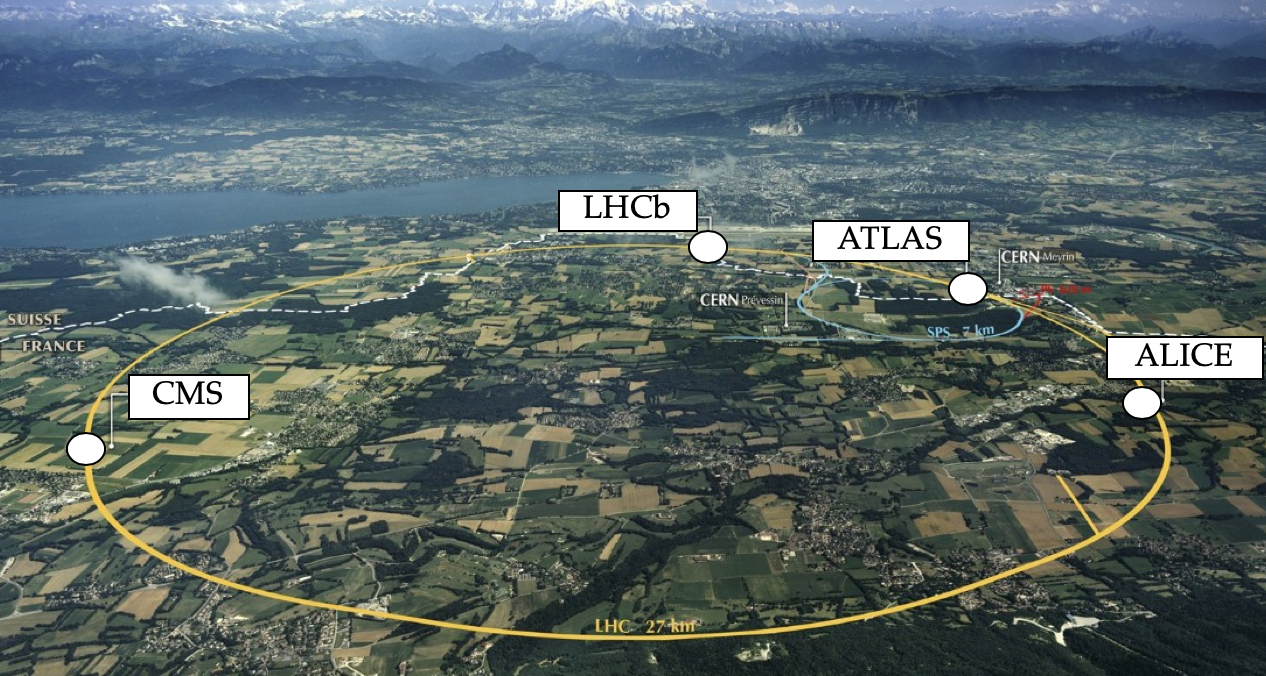
\includegraphics[width=15cm]{source/2-contextualizacao/images/LHC-now.png}
    \caption{Visão topográfica do \emph{CERN}.}
    \label{fig:cern-overview}
\end{figure}

O experimento \emph{LHCb} (\emph{Large Hadron Collider beauty}) tem como um dos principais objetivos tentar justificar o fato do universo ser aparentemente composto em quase sua totalidade de matéria, mas não de antimatéria \cite{cernsiteabout}. O experimento pretende encontrar respostas com a investigação de pequenas diferenças entre as duas, a partir do estudo de uma partícula chamada \emph{beauty quark}. O detector envolve cerca de 850 cientistas de 79 institutos de 18 países \cite{cernsitelhcb}, e sua estrutura está ilustrada na \ref{fig:lhcb-detector}. Foi implementado para este experimento o sistema \emph{LHCb Membership}, para gestão de pessoas, institutos e listas de autores. Este sistema foi utilizado como referência para o primeiro protótipo de testes automáticos desenvolvido neste trabalho.

\begin{figure}[H]
    \centering
    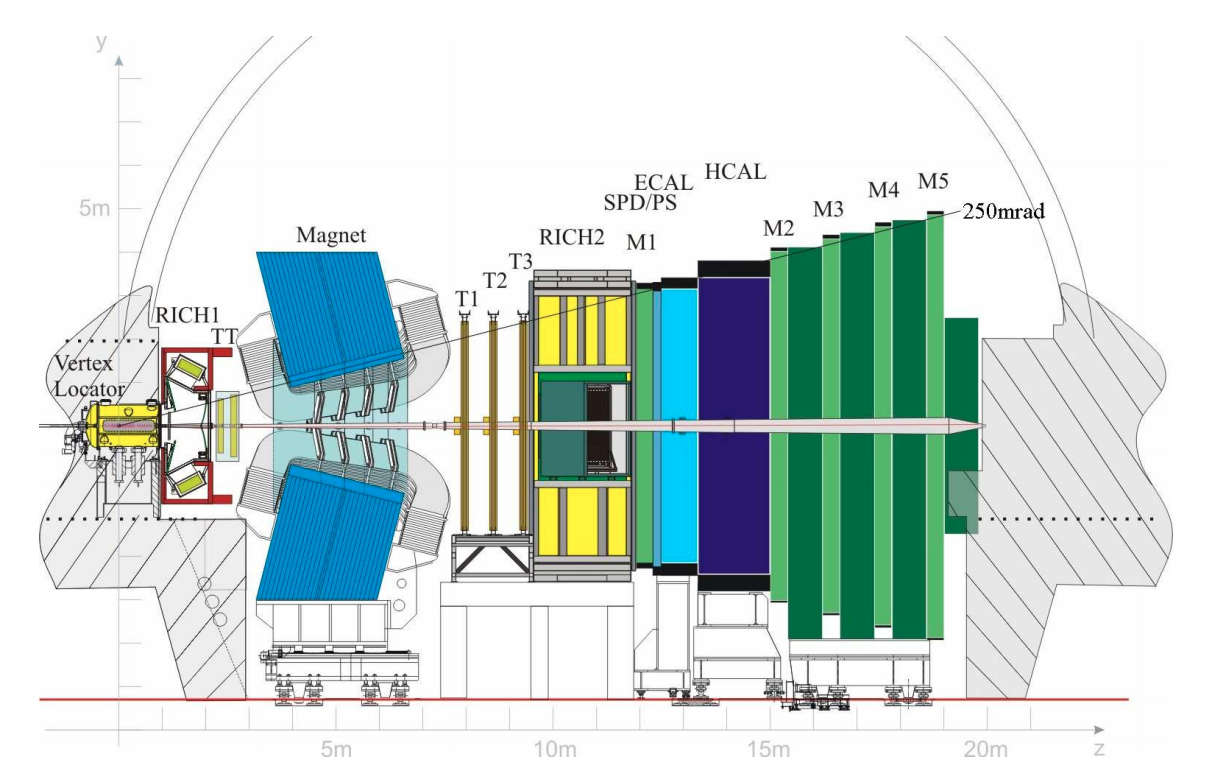
\includegraphics[width=14cm]{source/2-contextualizacao/images/lhcb-detector.png}
    \caption{Estrutura do detector \emph{LHCb} \cite{lhcb}.}
    \label{fig:lhcb-detector}
\end{figure}

O foco do detector ATLAS (\emph{A Toroidal LHC ApparatuS}) se concentra na tentativa de melhor entender os componentes fundamentais da matéria \cite{cernsiteatlas}. O detector investiga um vasto campo da física de partículas, desde o estudo das partículas subatômicas descritas no modelo padrão, até a busca por outras partículas, como por exemplo o bóson de Higgs e partículas que possam formar matéria escura. O experimento conta com 3000 autores científicos de 183 instituições presentes em 38 países \cite{cernsiteabout}, e foi constituído como apresentado na \ref{fig:atlas-detector}. Dos 22 sistemas desenvolvidos para este experimento, é valido destacar o sistema \emph{ACES}, \emph{Atlas Central Equipment System}, desenvolvido para gerenciamento de equipamentos e cabos, e planejamento de expansões no detector. Contando com mais de 150 mil equipamentos e 80 mil cabos, a complexidade deste sistema foi um motivacional para usá-lo como objeto de teste durante o desenvolvimento da plataforma, e atualmente este é o sistema que possui mais testes \emph{end-to-end}.

\begin{figure}[H]
    \centering
    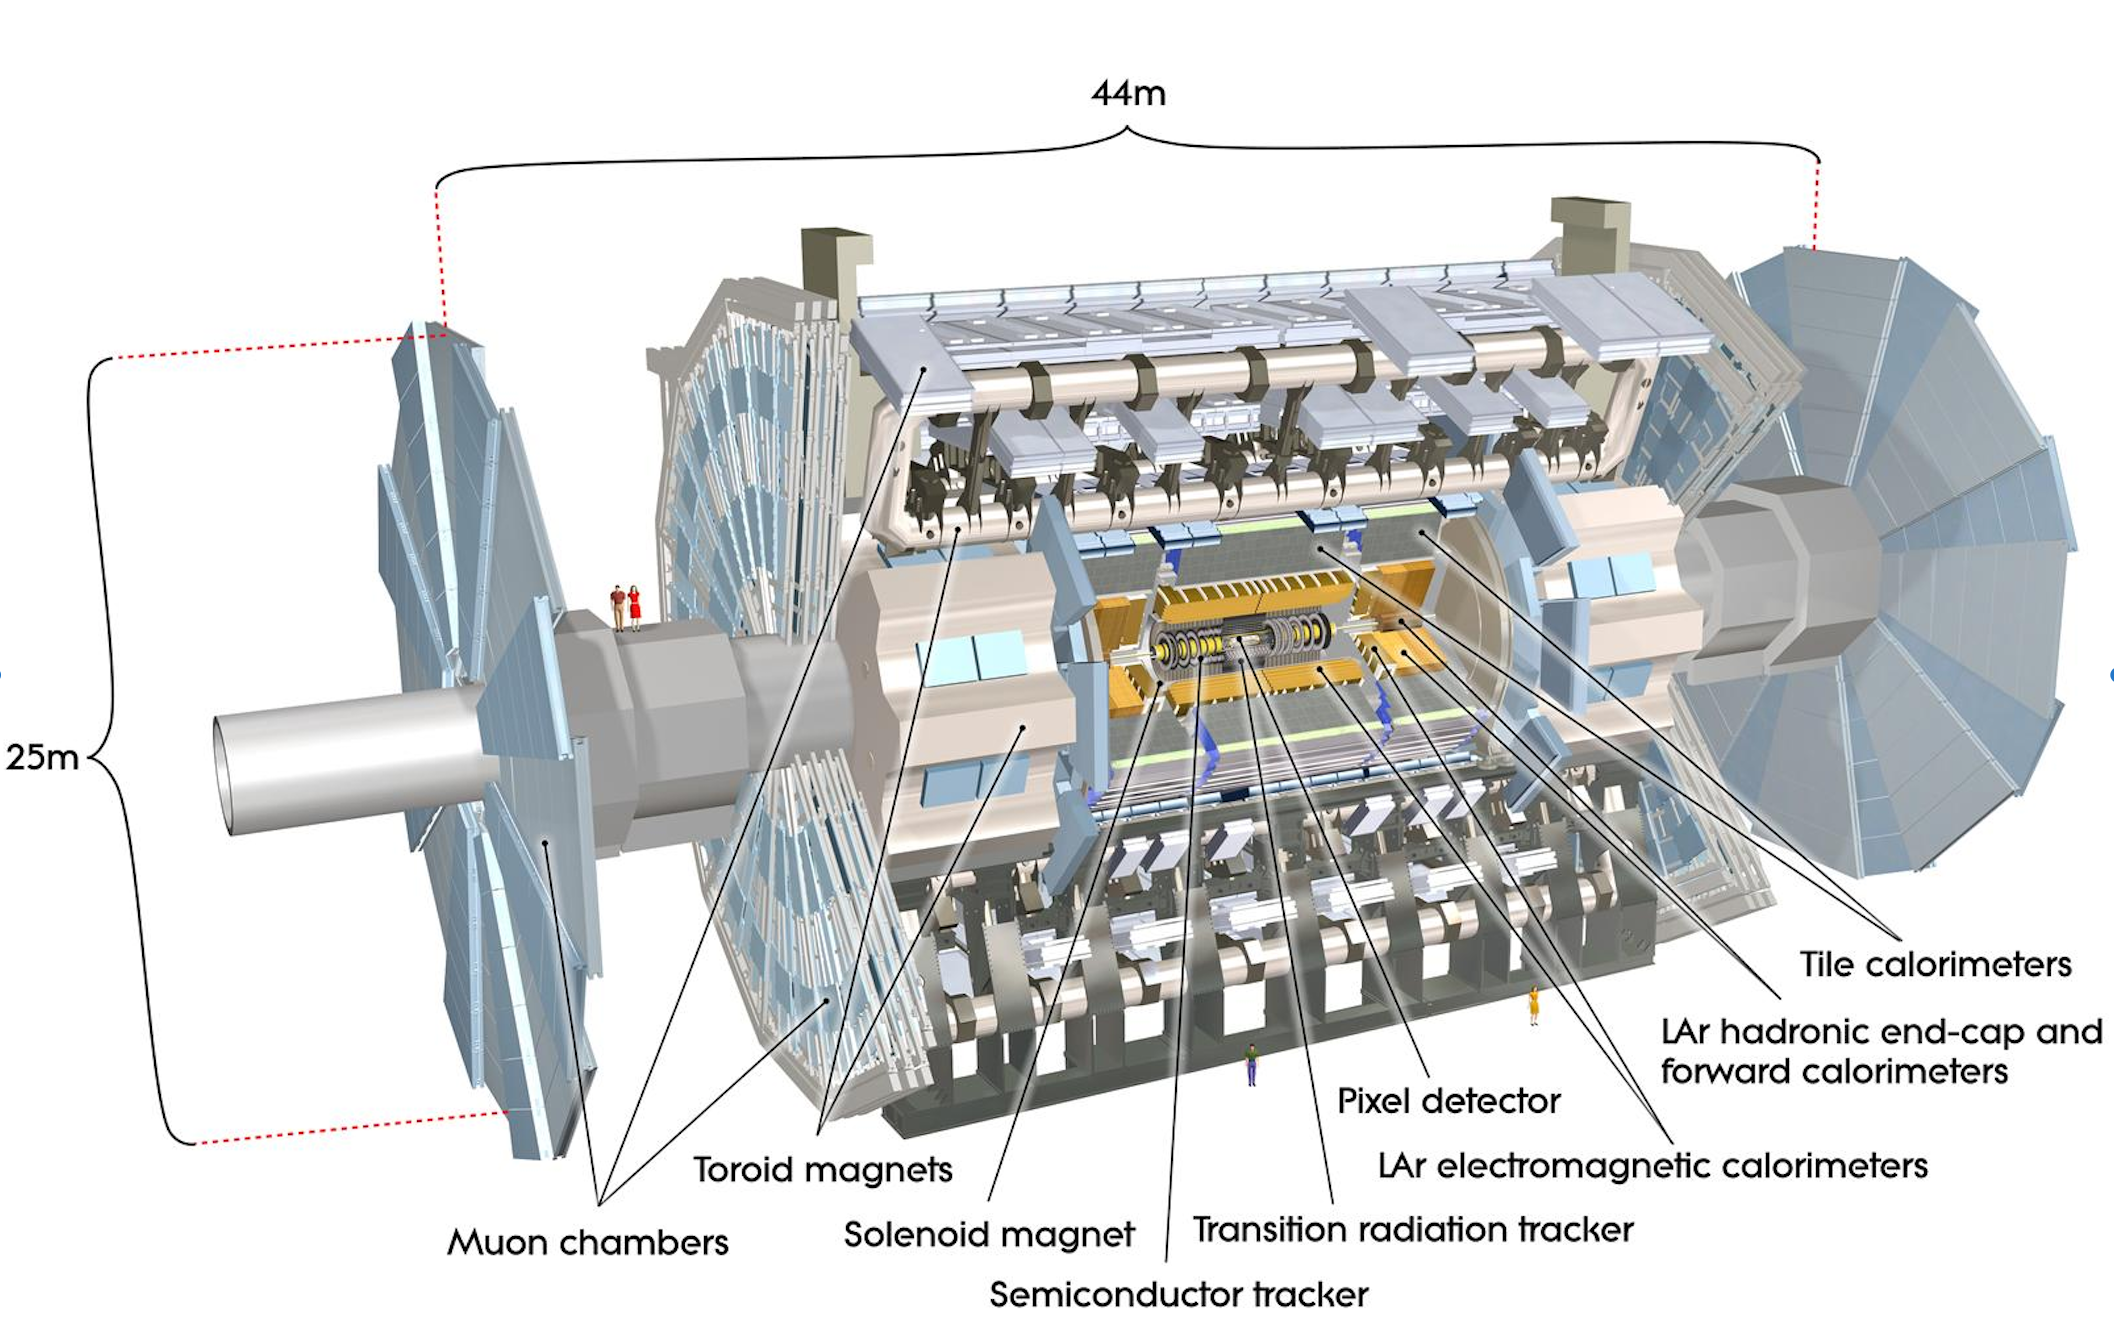
\includegraphics[width=14cm]{source/2-contextualizacao/images/atlas-detector.png}
    \caption{Estrutura do detector \emph{ATLAS} \cite{atlas}.}
    \label{fig:atlas-detector}
\end{figure}

Com a longevidade dos experimentos, as numerosas pesquisas realizadas pelo laboratório e a grande quantidade de pessoas envolvidas, um grande volume de dados vem sendo produzido desde as últimas décadas, e a complexidade exigida para o controle destes dados requer a assistência de softwares. É essencial para estes softwares possuírem fácil adaptação a mudanças, pois com os constantes aprimoramentos realizados nos experimentos, a grande rotatividade de contribuidores e a própria evolução do software, as necessidades de funcionalidades mudam com frequência. Isso se torna um forte motivacional para o investimento em testes de software, já que o dinamismo destes softwares exige verificações constantes quanto à confiabilidade oferecida.

Dentro do \emph{CERN}, diversos grupos atualmente desenvolvem soluções automatizadas para testes. Um exemplo é o grupo \emph{Joint Controls Project} que desenvolve softwares de sistemas de controle comuns aos 4 principais detectores. 
Juntamente com estes softwares, o grupo implementou um \emph{framework} próprio de escrita de testes unitários para verificá-los. Outro exemplo é o desenvolvimento de testes ponta a ponta para a plataforma \emph{EDH} que gerencia documentos eletrônicos do \emph{CERN}, feito pelo grupo \emph{Advanced Information Systems}. Em ambos casos as soluções apresentadas atingem propósitos específicos e em linguagens de programação distintas, não sendo soluções genéricas que atendam as necessidades de todos os grupos presentes no centro de pesquisa.